%---------------------------------------------------------------------
%
% Chapter 5: Formal Analysis of Multicriteria Algorithms
%
%---------------------------------------------------------------------
%
% ChapFormalAnalysis.tex
% Copyright 2015 Dr. Francisco J. Pulido
%
% This file belongs to the PhD titled "New Techniques and Algorithms for Multiobjective and Lexicographic Goal-Based Shortest Path Problems", distributed under the Creative Commons Licence Attribution-NonCommercial-NoDerivs 3.0, available in http://creativecommons.org/licenses/by-nc-nd/3.0/. The complete PhD dissertation is freely accessible from http://www.lcc.uma.es/~francis/
%
% This thesis has been written adapting the TeXiS template, a LaTeX template for writting thesis and other documents. The complete TeXiS package can be obtained from http://gaia.fdi.ucm.es/projects/texis/. TeXis is distributed under the same conditions of the LaTeX Project Public License (http://www.latex-project.org/lppl.txt). The complete license is available in http://creativecommons.org/licenses/by-sa/3.0/legalcode
%
%---------------------------------------------------------------------

\chapter{Formal Analysis of Multicriteria Algorithms}
\label{chapFormalAnalysis}

\begin{FraseCelebre}
\begin{Frase}
Make everything as simple as possible, but not simpler.
\end{Frase}
\begin{Fuente}
Albert Einstein (1879-1955)
\end{Fuente}
\end{FraseCelebre}
%
%\begin{resumen}
%

In this chapter we aim to give a formal analysis of the multiobjective algorithms introduced in Chapter \ref{chapContributions}. We look for the best algorithmic alternative when goal-based preferences are given by an user to characterize the optimal solution subset. Two possibilities arise here. The first, obvious one, is to calculate the whole Pareto set using a multiobjective search algorithm like \namoa \ and extract a posteriori the subset of Pareto solutions which satisfy the goals. A second alternative is to concentrate the search effort only in the goal-optimal solutions, i.e. discard from the first stages of the search those paths which will not lead to satisfy the goals or minimize the deviation from them. This thesis has introduced one such algorithm, called \lexgo. 
%a multicriteria search algorithm developed to concentrate search effort on goal-optimal solutions.

Both algorithms, \namoa \ and \lexgo \ may share the same label selection procedure and filtering/pruning processes, though \lexgo \ introduces extra processes of pruning and filtering considering the deviation from goals, which will be formally studied further in this section. 

Another algorithmic contribution introduced in Chapter \ref{chapContributions} is the introduction of a new method, t-discarding, to speed up dominance checks. This method can be applied to the pruning and filtering checks keeping the admissibility of the algorithm. This technique has been applied to multiobjective and goal-based search, yielding two new algorithms: 
\namoate \ and \lexgote. Their properties are also analyzed in this section. 

We organize the relevant formal properties for a multicriteria search algorithm as follows: 

\begin{description}
    \item[Admissibility] 

All algorithms introduced in this thesis are theoretically proven to be admissible. The formal proofs on the admissibility of \namoa \ were presented in \citep{Mandow2005, Mandow2010}. \lexgo \ properties of admissibility will be presented further in Section \ref{chapFormalAnalysis:sec:analysisLEXGO}. Finally, the t-discarding technique which is employed in \namoate \ and \lexgote \ is analyzed in Section \ref{chapFormalAnalysis:sec:analysisNAMOATE}. 

    \item[Efficiency] 

A standard in formal analyses to measure the efficiency of multicriteria search algorithms is the number of explored labels. A recent study showed that \namoa \ is optimal according to this measure when used with consistent lower bounds \citep{Mandow2010}. \namoa \ has been shown to expand an equal or smaller number of labels when using more informed consistent lower bound functions \citep{Mandow2010}. \lexgo, in particular, always expands a subset of the labels expanded by \namoa, see Section \ref{chapFormalAnalysis:sec:efficiencyLexgo} for further details. 

The number of explored labels can be a good measure of the space requirements of the algorithms. However, in multicriteria search the time requirements are influenced by other factors as well. The algorithms that use t-discarding expand the same set of labels as the traditional ones. However, the experimental evaluation reveals that the time performance is greatly improved. Therefore, we also analyze another important measures for the time performance of multicriteria search, the number of dominance comparisons and the cardinality of the non-dominated sets used to check dominance. These are the key of the impressive performance of the t-discarding technique. 

\end{description}

This chapter is organized as follows. Section \ref{chapFormalAnalysis:sec:analysisNAMOA} summarizes formal properties of \namoa. The same aspects are comparatively analyzed for \lexgo \ in Section \ref{chapFormalAnalysis:sec:analysisLEXGO}. Finally, the t-discarding technique is formally proved to be time efficient and characterized employing \namoate \ and \lexgote \ as examples of use. Finally, a brief discussion is presented. 

%-------------------------------------------------------------------
\section{Formal characterization of \texorpdfstring{\namoa}{NAMOA*}}
\label{chapFormalAnalysis:sec:analysisNAMOA}
%-------------------------------------------------------------------

The formal properties of \namoa \ have been recently introduced by \citet{Mandow2010} and further studied by \citet{Machuca2012a}. In this section, 
we briefly review previous theoretical properties of \namoa, since it is the basis on which \lexgo \ has been devised. This will allow us to analyze only the new features brought by \lexgo, the t-discarding technique and their implications on the admissibility and efficiency.

%-------------------------------------------------------------------
\subsection{Admissibility}
\label{chapFormalAnalysis:sec:admissibilityNamoa}
%-------------------------------------------------------------------

The results that follows are taken from  \citet{Mandow2010} and \citet{Machuca2012a}.

\begin{property}[Admissibility]\label{chapFormalAnalysis:prop:multiObjAdmissibilityNamoa}

When the graph $G=(N,A)$ is locally finite and $H(n)$ is a lower bound (admissible) the search is considered \textbf{admissible}, i.e. it is guaranteed to find \textbf{all non-dominated} optimal solutions, or does not terminate if there are infinite solutions. \namoa \ is admissible even on infinite graphs with some additional assumptions:

\begin{description}\label{chapFormalAnalysis:eq:multiObjAdmissibilityCondNamoa}
  \centering      
\item[a)] 
$\forall n \in N \land \forall \vec h =(h_1,\ldots ,h_q) \in H(n), \quad \forall k \in [1,q], \ h_k(n) \geq 0$
	 \item[b)] 
$\forall (n,n') \in A,  \land \forall \vec  c(n,n') \in \vec c, \quad \forall k \in [1,q], \ c_k(n,n') \ \geq \epsilon > 0$  
\end{description}
\end{property}

Several important properties of \namoa \ follow. These are analogous to those of the single objective A$^*$ algorithm.

\begin{teorema} \label{chapFormalAnalysis:teo:multiObjAdmissibility-teorema1Namoa} \citep[Theorem 4.2]{Mandow2010}
 For each non-dominated solution path
  $P^*=(s, n_1,\ldots, n_i, n_{i+1}\ldots \gamma)$ with cost $\vec
  g(P^*) = \vec c^{~*}$, there is always before its discovery a subpath
  $P_{i}^*=(s, n_1, \ldots,n_i)$  of $P^*$ such that: 
\begin{description}
  \centering  
    \item[a)]$P_{i}^*$ is recorded in $SG$
    \item[b)]$\ \vec g(P_{i}^*) \in G_{op}(n_i)$ \ \ \ \ \ \ \
    \item[c)]$\exists  \vec f \in F(P_{i}^*) \ | \ \vec f \preceq \vec c^{~*}$
\end{description}
That is to say the algorithm never discards Pareto optimal solutions.

\end{teorema}

\begin{teorema} \label{chapFormalAnalysis:teo:multiObjAdmissibility-teorema2Namoa} 
\citep[Theorem 4.3]{Mandow2010}
If there is at least a solution path $P^*$, the algorithm terminates even on infinite graphs.
\end{teorema}

\begin{corolario} \label{chapFormalAnalysis:corol:multiObjAdmissibility-corolario1Namoa} 
\citep[Corollary 4.4]{Mandow2010}
Whenever there is at least a solution path $P^*$, the set of non-dominated solution costs $C^*$ is finite.
\end{corolario}

\begin{lema}\label{chapFormalAnalysis:lem:multiObjAdmissibility-lema1Namoa} 
\citep[Lemma 4.5]{Mandow2010}
Each path $P \in \mathbb{P}_{sn}$  selected from $OPEN$ for expansion
  satisfies upon selection that,
\begin{equation}
%$
\exists \vec h \in H(n) \quad | \quad \nexists \vec c^{~*} \in C^*,
  \quad \vec c^{~*}\prec
  \vec g(P) + \vec h
%$
\end{equation}
\end{lema}

\begin{teorema}\label{chapFormalAnalysis:teo:multiObjAdmissibility-teorema4Namoa} 
\citep[Theorem 4.6]{Mandow2010}
A dominated solution can never be selected for expansion.
\end{teorema}

\begin{corolario} \label{chapFormalAnalysis:corol:multiObjAdmissibility-corolario2Namoa} 
\citep[Corollary 4.7]{Mandow2010}
The set of found solution vectors, COSTS, is at any time a subset of the set of all non-dominated solution cost vectors, i.e. $COSTS \subseteq C^*$.
\end{corolario}

\begin{teorema}\label{chapFormalAnalysis:teo:multiObjAdmissibility-teorema5Namoa} 
\citep[Theorem 4.9]{Mandow2010}
Since \namoa \ satisfies all the above conditions, \namoa \ is admissible.
\end{teorema}

Admissibility (i.e. the algorithm is exact and returns the whole set of solutions to the problem) is an important property. However, it is also important to prove that the efficiency of the algorithm improves with more precise lower bounds. 

%-------------------------------------------------------------------
\subsection{Efficiency of lower bounds and optimality}
\label{chapFormalAnalysis:sec:efficiencyNamoa}
%-------------------------------------------------------------------

Pathological behavior has been observed in another multiobjective search algorithm called \moa \ \citep{stewartwhite1991}. Although \moa \ is admissible, it has been proven to decrease performance in certain cases with more informed lower bounds \citep{PerezdelaCruz2013}. Fortunately, \namoa \ has been proven to enjoy efficiency properties analogous to those of \astar.

\begin{defi}\label{chapFormalAnalysis:def:multiObjc-acotado}
\citep[Definition 5.1]{Mandow2010}
A path $P= (s = n_0, n_1, n_2,\ldots, n_k)$ is said to be
\textbf{C-bounded} with respect to $H(n)$ (or C(H)-bounded) if for all subpaths $P_i =(n_0, n_1,\ldots,n_i)$ of $P$ it holds that:
\begin{equation}
\exists \vec h \in H(n_i) \quad | \quad \nexists \vec c \in C, \quad
\vec c \prec \vec g(P_i) + \vec h   
\end{equation}
\end{defi}

By definition, a $C^*$-bounded path will never be filtered (see Lemma \ref{chapFormalAnalysis:lem:multiObjAdmissibility-lema1Namoa} and Theorem \ref{chapFormalAnalysis:teo:multiObjAdmissibility-teorema4Namoa}). Therefore, such paths will be either selected for expansion or pruned.

\begin{teorema}\label{chapFormalAnalysis:teo:multiObjAdmissibility-teorema6Namoa}
\citep[Theorem 5.9]{Mandow2010} 
If $H(n)$ is consistent, then a \textbf{necessary and sufficient} condition
for \namoa \ to select some path $P =(s,\ldots,n)$ for expansion is
that: 
\begin{description}
  \centering  
    \item[a)]$P$ be a non-dominated path from $s$ to $n$
    \item[b)]$P$ be $C^*$-bounded \quad \quad  \quad \quad \quad \quad \quad \quad \quad \quad \
\end{description}
\end{teorema}

\begin{teorema}\label{chapFormalAnalysis:teo:multiObjAdmissibility-teorema7Namoa}
\citep[Theorem 5.10]{Mandow2010} 
 Let $H_1(n)$ and $H_2(n)$ be two admissible lower bounds for the same
  problem. Let $H_2(n)$ be additionally \textbf{monotone}. Let
  $NAMOA^*_1$ and $NAMOA^*_2$ be two versions of \namoa \ that differ
  only in the use of different lower bound functions $H_1(n)$ and $H_2(n)$
  respectively. If $H_2(n)$ is at least as informed as $H_1(n)$, then
  \textbf{all} paths selected for expansion by $NAMOA^*_2$ will also be
  selected for expansion by $NAMOA^*_1$.
\end{teorema}

\begin{property}[Efficiency]\label{chapFormalAnalysis:prop:multiObjEfficiency}

When $\forall n \in N, \  H(n) = \{ \vec 0 \}$, \namoa \ is analogous to the blind algorithm of \citet{Martins1984} or \citet{Raith2009}. When $H(n)$ is \textbf{consistent} or \textbf{monotone}, only the strictly necessary $C^*$-bounded paths will be expanded, and the pruning of those $C^*$-bounded paths not belonging to non-dominated solutions will be maximal, analogously to the single-objective case. If the costs of some optimal solution is denoted by vectors $\vec c^{~*}$, \namoa \ will always expand for sure all labels with some $\vec f(n) \prec \vec  c^{~*}$. Given consistent lower bound functions,  more actual suboptimal alternatives can be pushed out of the Pareto frontier with \textbf{more informed} lower bounds, reducing search effort.
\end{property}

\begin{property}[Optimality]\label{chapFormalAnalysis:prop:multiObjOptimality}
\namoa \ has been proved to be optimal in the number of path expansions among the class of exact best-first algorithms when using consistent distance estimates \citep{Mandow2010}, i.e. no algorithm in this class provided only with the same information could avoid exploring a single label explored by \namoa \ without compromising admissibility.
\end{property}

%-------------------------------------------------------------------
\section{Formal characterization of \texorpdfstring{\lexgo}{LEXGO*}}
\label{chapFormalAnalysis:sec:analysisLEXGO}
%-------------------------------------------------------------------

This section proves some relevant properties of \lexgo. First, we will show that \lexgo \ is at least as \emph{efficient} as \namoa \ in terms of label expansions, i.e. it always expands a subset of the labels expanded by \namoa. Then, we will show that it is \emph{admissible}, i.e. it always returns the set of all goal-optimal solutions. Again, these properties are analogous to those of the single objective \astar \ search algorithm. 

The proofs presented in this section rely on a set of reasonable
assumptions, analogous to those presented in Section  \ref{chapFormalAnalysis:sec:admissibilityNamoa} to prove the admissibility of \namoa \ and other multiobjective label-setting algorithms:

\begin{supo}\label{supo-lexgo1}
The graph $G = (N,A)$ to be searched is locally finite, i.e. only a finite number of arcs emanate from each node.
\end{supo}

\begin{supo}\label{supo-lexgo2}
The lower bound function $\vec{h}(n)$ is consistent.
\end{supo}

%-------------------------------------------------------------------
\subsection{Efficiency}
\label{chapFormalAnalysis:sec:efficiencyLexgo}
%-------------------------------------------------------------------

Let us consider first the question of efficiency. \lexgo \ is essentially a version of \namoa \ with additional pruning and filtering rules. However, simply adding additional discarding rules to \namoa \ does not necessarily guarantee that the resulting algorithm will explore a subset of the labels expanded by \namoa. The example in Figure \ref{fig:5-1} illustrates the case for an arbitrary pruning rule. Let us assume $\forall n \ \ \vec h(n) = \vec 0$. There are two non-dominated paths from $s$ to $n_1$ with costs (8,6) and (9,1), respectively. Let us assume that by a certain arbitrary rule the path with cost (8,6) prunes the one with cost (9,1). There are two paths from $s$ to $n_2$ through $n_1$ with costs (9, 14) and (10, 9). The latter dominates the path from $s$ to $n_2$ with cost (10,10). However, due to the pruning rule, it will never be generated, and the dominated path with cost (10,10) will need to be expanded. In other words, the inclusion of an arbitrary pruning rule may lead to the exploration of labels never considered by \namoa.

\begin{figure}[!ht]
\centering
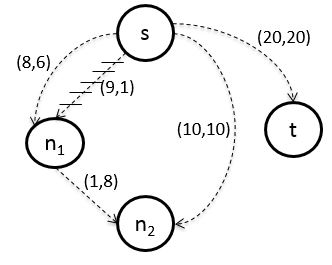
\includegraphics[width=0.4\textwidth]{Images/Chapter5/naive-pruning-example}
\caption{A pruning rule prunes a path to $n_1$ with cost (9,1) leading to the expansion of the dominated label (10,10) in $n_2$.}
\label{fig:5-1}
\end{figure} 

So we must formally show that the additional rules of \lexgo \ guarantee that only a subset of the labels expanded by \namoa \ are actually considered. To do so, Lemma \ref{lema:pruning1} analyzes the relation between pruning, goal, and Pareto preferences. Then, Theorem \ref{teo:subset} proves the desired efficiency of \lexgo, and finally, Theorem \ref{chapFormalAnalysis:teo:lexgo-admissible} establishes its admissibility.

\begin{lema}\label{lema:pruning1} 
Assume $\vec{\epsilon} \succeq \vec{0}$. Then

a) If $\vec{y} \prec_{P} \vec{y'}$  then $\vec{y} + \vec{\epsilon} \prec_{G} \vec{y'} + \vec{\epsilon}$.

b) If $\vec{y} \prec_{P} \vec{y'}$  then $\vec{y} + \vec{\epsilon} \prec_{P} \vec{y'} + \vec{\epsilon}$.

c) If $\vec{y} \prec_{P} \vec{y'}$ and $\vec{y'} \prec \vec{y''}$, then $\vec{y} \prec_{P} \vec{y''}.$

\end{lema}

\begin{demo}
Notice that, by definition,

\begin{equation}
\delta_i(\vec y, \vec{y'}) = 0 \quad \Rightarrow \quad \forall k \in I_i \hspace{3mm} s_k \geq s'_k
\label{eq:lexgo-pruning-a}
\end{equation}

Additionally, assume $d_i(\vec y) = d_i(\vec{y'})$. Since $\vec y$ has greater or equal slack than $\vec{y'}$ for all goals in level $i$, then it is straightforward that,

\begin{equation}
\forall \vec{\epsilon} \succeq \vec{0}, \quad d_i(\vec{y'} + \vec{\epsilon}) \geq  d_i(\vec{y} + \vec{\epsilon})
\label{eq:lexgo-pruning-b}
\end{equation}

Notice again that, by definition, 

\begin{equation}
\delta_j(\vec y, \vec{y'}) < d_j(\vec{y'}) - d_j(\vec{y}) \quad \Rightarrow \quad \forall \vec{\epsilon} \succeq \vec{0}, \quad d_j(\vec{y'} + \vec{\epsilon}) >  d_j(\vec{y} + \vec{\epsilon})
\label{eq:lexgo-pruning-c}
\end{equation}

Property (a) follows then from the definition of goal preferences. Assume $\vec{y} \prec_{P} \vec{y'}$, and that $\exists j \quad d_j(\vec y) < d_j(\vec{y'}) \land (\forall i < j \quad d_i(\vec y) = d_i(\vec{y'}))$. 
Then, from equations \ref{eq:lexgo-pruning-b} and \ref{eq:lexgo-pruning-c}, $\vec{y'} + \vec{\epsilon}$  will not have better deviation over $\vec{y} + \vec{\epsilon}$ for any of the first $j$ levels, and will have strictly worse deviation for at least one of them, i.e. $\vec{y} + \vec{\epsilon} \prec_{G} \vec{y'} + \vec{\epsilon}$.

For part (b) we still have to prove the additional constraints imposed on cross-slacks. Let us denote by $s''_k$ and $s'''_k$ the slack for goal $k$ of vectors $\vec{y} + \vec{\epsilon}$ and $\vec{y'} + \vec{\epsilon}$ respectively. For all levels $i<j$ we have,
\begin{align*}
\delta_i(\vec y, \vec{y'}) = 0 \quad \Rightarrow \quad \forall k \in I_i \ s_k \geq s'_k \ \ \Rightarrow \ \ \forall k \in I_i \hspace{3mm} s''_k \geq s'''_k \ \ \Rightarrow \ \ \delta_i(\vec y + \vec{\epsilon}, \vec{y'}+ \vec{\epsilon}) = 0
\label{eq:lexgo-pruning-f}
\end{align*}

\noindent and also $d_i(\vec {y'} + \vec{\epsilon}) \geq d_i(\vec {y}+ \vec{\epsilon})$. 

If for some $m < j$ \ \ $d_m(\vec {y'} + \vec{\epsilon}) > d_m(\vec {y}+ \vec{\epsilon})$, then $\delta_m(\vec y + \vec{\epsilon}, \vec{y'}+ \vec{\epsilon}) = 0 < d_m(\vec {y'} + \vec{\epsilon}) - d_m(\vec {y}+ \vec{\epsilon})$, and the property holds. Otherwise, we need to prove that the condition on cross-slacks still holds for level $j$. Let us define $\delta^i(\vec{y}, \vec{y'}) = w_i \times \max(0, s'_i - s_i)$. The following is an alternate definition of formula \ref{eq:slack-var},
\begin{align*}
    \delta_j(\vec{y}, \vec{y'}) = \sum_{m\in I_j} \delta^m(\vec{y}, \vec{y'})
 \end{align*}
	
Analogously, let us define $d^i(\vec{y}) = w_i \times \max(0, y_i - t_i)$. Then,
\begin{align*}
    d_j(\vec{y}) = \sum_{m\in I_j} d^m(\vec{y})
\end{align*}
	
Now, we analyze for each goal $m \in I_j$ its influence in deviations and cross-slack. We have three cases to consider:

\begin{itemize}
	\item When $s_m = s'_m$, deviations increase in the same amount (i.e. their relative difference does not change) and $\delta^m(\vec{y}+ \vec{\epsilon}, \vec{y'}+ \vec{\epsilon}) = \delta^m(\vec{y}, \vec{y'}) = 0$.

	\item If $s_m > s'_m$, then $d^m(\vec{y'}) - d^m(\vec{y}) \leq d^m(\vec{y'} + \vec \epsilon) - d^m(\vec{y} + \vec \epsilon)$, i.e. the relative difference between deviations can never decrease. Since $\delta^m(\vec{y}, \vec{y'}) = \delta^m(\vec{y}+ \vec{\epsilon}, \vec{y'}+ \vec{\epsilon})$ , the condition will hold for the goal.

	\item If $s_m < s'_m$, then we have to consider three distinct cases:
	\begin{itemize}
		\item When $0 \leq \epsilon_m \leq s_m < s'_m$, both deviations are zero, their relative difference remains zero and $\delta^m(\vec{y},\vec{y'})$ does not change.
		\item When $ s_m < \epsilon_m \leq s'_m$, we have $[d^m(\vec{y'}) - d^m(\vec{y}) ] - [d^m(\vec{y'} + \vec\epsilon) - d^m(\vec{y} + \vec\epsilon)] = w_m \times (\epsilon_m - s_m)$. However, we also have $\delta^m(\vec{y},\vec{y'}) - \delta^m(\vec{y} + \vec\epsilon,\vec{y'}+ \vec\epsilon) = w_m \times (\epsilon_m - s_m)$, i.e. it decreases in the same amount as before, and the inequality still holds for goal $m$. 
		\item When $ s_m  < s'_m < \epsilon_m$, we have $[d^m(\vec{y'}) - d^m(\vec{y}) ] - [d^m(\vec{y'} + \epsilon) - d^m(\vec{y} + \epsilon)] = w_m \times (s'_m - s_m)$. However, $\delta^m(\vec{y},\vec{y'}) - \delta^m(\vec{y} + \vec\epsilon,\vec{y'}+ \vec\epsilon) = w_m \times (s'_m - s_m)$, i.e. it also decreases in the same amount as before, and the inequality still holds for goal $m$. 
		\end{itemize}
\end{itemize}

Part (c) is quite straightforward. Notice that,
\begin{equation}
\vec{y'} \prec \vec{y''}  \Rightarrow  \forall l \forall k \in I_l \quad s'_k \geq s''_k
\label{eq:lexgo-pruning-d}
\end{equation}
If  $\vec{y} \prec_{P} \vec{y'}$, then we have that for all levels $i<j$, $\delta_i(\vec y, \vec{y'}) = 0$, 
$\delta_i(\vec y, \vec{y''}) = 0$, and $d_i(\vec{y''}) \geq d_i(\vec{y'}) = d_i(\vec{y})$. 

Let us examine level $j$. From equation \ref{eq:lexgo-pruning-d} it follows that $\delta_j(\vec y, \vec{y'}) \geq \delta_j(\vec y, \vec{y''})$ and from dominance $d_j(\vec{y''}) \geq d_j(\vec{y'})$. In consequence,

\begin{equation}
d_j(\vec{y''}) - d_j(\vec{y}) \  \geq \ d_j(\vec{y'}) - d_j(\vec{y}) \ > \ \delta_j(\vec y, \vec{y'}) \  \geq \ \delta_j(\vec y, \vec{y''})
\label{eq:lexgo-pruning-e}
\end{equation}

\noindent and therefore $\vec{y} \prec_{P} \vec{y''}$. $\Box$

\end{demo}

\begin{teorema}\label{teo:subset}
When the lower bound function is monotone \lexgo \ explores a subset of the labels explored by \namoa, i.e. if \namoa \ does not explore a label $(n, \vec g)$, \lexgo \ will not explore it either.
\end{teorema}

\begin{demo}
A label $(n, \vec g, \vec f)$ is not explored by \namoa \ if (a) $\exists \vec{c^*} \in C^*$ such that $\vec{c^*} \prec \vec f$, or (b) $\vec g$ is dominated in $n$. 

It is straightforward that \lexgo \ never explores a label discarded by  \namoa \ by condition (a). Since  $C^*_G \subseteq C^*$, for all $c^* \in C^*$, either $c^* \in C_G^*$, or $\vec d_B = \vec{d^*} \prec_L \vec d(\vec{c^*})$. In the latter case, if for some $\vec f$, $\vec{c^*} \prec \vec f$, then $\vec{d^*} \prec_L \vec d(\vec{c^*}) \preceq_L \vec d(\vec f)$. Therefore, \lexgo \ filters the labels with equations \ref{eq:cond-filter-dom} and \ref{eq:cond-filter-new}.  

Let us consider now labels discarded by \namoa \ by condition (b). Let us assume a non-dominated path $P = (s, n, \ldots, n_i, \ldots, n_k)$ to $n_k$ represented by label $(n_k, \vec g, \vec f)$, and its two subpaths $P_1 = (s, n, \ldots, n_i)$ and $P_2 = (n_{i+1}, \ldots, n_k)$. Let us also assume a dominated path $P' = (s, \ldots, n_k)$ to $n_k$ in OPEN with label $(n_k, \vec{g'}, \vec{f'} )$.  Finally, lets assume that $P_1$ is the largest subpath of $P$ to enter OPEN, with label $(n_i, \vec g_1, \vec f_1)$. This situation is depicted in  Figure \ref{fig:4-2-prune}.

Let us assume label $(n_i, \vec g_1, \vec f_1)$ is in OPEN. Since the lower bound function is monotone, as defined in the assumptions, \ $\vec g_1 + \vec h_i \preceq \vec g + \vec h_k \prec \vec{g'} + \vec h_k$ and $P'$ can never be selected by \lexgo. If eventually, $n_i = n_k$ $P'$ is dominated and pruned by $P$.

On the other hand, if $(n_i, \vec g_1, \vec f_1)$ is never selected and not in OPEN, then there must be some other path $P_3$ that pruned $P_1$, i.e. $\vec f(P_3) \prec_P \vec f(P_1)$. By Lemma \ref{lema:pruning1}(b), we have $\vec f(P_3P_2) \prec_P \vec f(P_1P_2)$. This fact, together with the fact that $\vec f(P_1P_2) \prec \vec f(P')$, leads us to conclude by virtue of Lemma \ref{lema:pruning1}(c), that  $\vec f(P_3P_2) \prec_P \vec f(P')$, i.e. if a path prunes some other non-dominated path, then the extensions of the former will also prune those that would be pruned by the latter. Therefore, the property holds.$\Box$  

\begin{figure}[!ht]
\centering
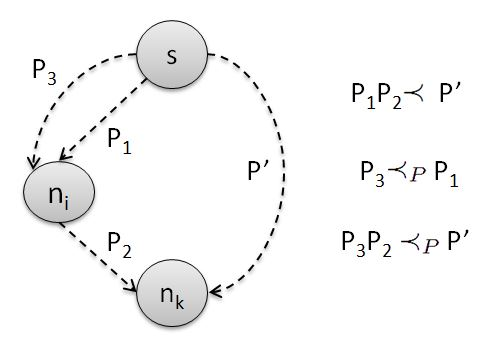
\includegraphics[width=0.4\textwidth]{Images/Chapter5/prune}
\caption{Scenario where a dominated path $P'$ is pruned either by $P_1P_2$ or $P_3P_2$.}
\label{fig:4-2-prune}
\end{figure} 

\end{demo}

%-------------------------------------------------------------------
\subsection{Admissibility}
\label{chapFormalAnalysis:sec:admissibilityLexgo}  
%-------------------------------------------------------------------

Once the efficiency of \lexgo \ has been established, we turn our attention to admissibility, i.e. to prove that the subset of labels explored by \lexgo \ still includes all goal-optimal solutions. A scalar algorithm is said to be \emph{admissible} if it is guaranteed to return an optimal solution whenever a solution exists. We extend the definition as follows: a multiobjective search algorithm with goal-based preferences is \emph{admissible} if it terminates with the set of \emph{all} goal-optimal solutions to the problem. 

\begin{teorema} \label{chapFormalAnalysis:teo:lexgo-admissible}
Algorithm \lexgo \ is admissible.
\end{teorema}

\begin{demo}
\lexgo \ is a label-setting algorithm that generates partial paths from the start node to the destination. Each partial path is either expanded, filtered, or pruned. A goal-optimal solution could be pruned by pruning conditions \ref{eq:cond-prune-dom} or \ref{eq:cond-prune-deviation} as described in Section \ref{subsubsec:Pruning-conditions}, or could be filtered by filtering conditions \ref{eq:cond-filter-dom} or \ref{eq:cond-filter-new} from Section \ref{subsubsec:Filtering-conditions}. By definition, a goal-optimal solution has a non-dominated cost. Since the optimality principle holds for dominated costs, neither pruning condition \ref{eq:cond-prune-dom} nor filtering condition \ref{eq:cond-filter-dom} will ever discard a goal-optimal solution.

The proof for condition \ref{eq:cond-prune-deviation} follows. Let us assume two paths $P^1=(s,\ldots,n)$ and $P^2=(s,\ldots,n)$, leading to the same node $n$, and an additional Pareto-optimal path $P^3 =(n,\ldots,t)$ leading from $n$ to a destination node. Let us call $\vec{f^1} = \vec{f}(P^1) = \vec g(P^1) + \vec{h}(n)$, 
$\vec{f^2} = \vec{f}(P^2) = \vec g(P^2) + \vec{h}(n)$.
Since the lower bound is optimistic, we know that $\vec{h}(n) \preceq \vec g(P^3)$. Let us call $\vec{e} = \vec g(P^3) - \vec{h}(n) \succeq \vec{0}$.
Extending $P^1$ and $P^2$ with $P^3$, the costs of both solutions are
respectively $\vec{f^{13}}= \vec g(P^1) + \vec g(P^3) = \vec g(P^1) + \vec{h}(n) + \vec{e} = \vec{f^1} + \vec{e}$ \ and $\vec{f^{23}}= \vec g(P^2) + \vec g(P^3) = \vec g(P^2) + \vec{h}(n) + \vec{e} = \vec{f^2} + \vec{e}$.

Let us assume that $P^1$ prunes $P^2$ in virtue of condition \ref{eq:cond-prune-deviation}. Then $\vec{f^1} \prec_P\vec{f^2}$ and, by Lemma \ref{lema:pruning1}(a), $\vec{f^{13}} = \vec{f^1} + \vec{e} \prec_G \vec{f^2} + \vec{e} = \vec{f^{23}}$, so by this expansion $P^2$ does not lead to a better solution than $P^1$. Since no assumptions were made about $P^3$, the result holds for every expansion of $n$, therefore $P^2$ does not lead to a better solution than $P^1$ and the pruning is correct.

Finally, let us consider filtering condition \ref{eq:cond-filter-new}, due to the lexicographic selection policy, the deviation of the first solution found $\bestd = \vec d_t$ is trivially equal or lexicographically better than the deviation of any other label in OPEN. No goal-optimal solution cost $\vec{c^*} \in C_G^*$ with deviation $\vec d(\vec{c^*})$ can have worse lexicographical deviation than $\bestd$
%, $\bestd \nprec_L \vec d(\vec{c^*})$, otherwise $\vec g_t \prec_G \vec{c^*}$ and it could not be a goal-optimal solution. 
Therefore, filtering condition \ref{eq:cond-filter-new} never filters goal-optimal solutions.

Since \lexgo \ never prunes nor filters goal-optimal solutions, the only remaining possibility is that they are all selected and found before termination, i.e. \lexgo \ is admissible.$\Box$
\end{demo}

%-------------------------------------------------------------------
\section{Formal characterization of \texorpdfstring{\namoate}{NAMOA*te}}
\label{chapFormalAnalysis:sec:analysisNAMOATE}
%-------------------------------------------------------------------

This section proves some relevant properties of \namoate \ under reasonable assumptions. The t-discarding method, see Section \ref{chapMultiObjAlg:sec:Time-efficient-MSalg}, introduces a new technique to check dominance of new alternatives against the solutions already found (filtering) and against partial paths to each node already explored (cl-pruning). We will show that \namoa \ is not affected when the t-discarding technique is applied instead of the standard dominance tests. 

%-------------------------------------------------------------------
\subsection{Admissibility}
\label{chapFormalAnalysis:sec:admissibilityNamoate}
%-------------------------------------------------------------------

In order to demonstrate the admissibility of \namoate, we will make the following assumptions:

\begin{supo} \label{supo:1}
The lower bound function returns a single vector estimate for each node, i.e. $H(n) = \{  \vec h(n) \}$, and satisfies the monotone property.
\end{supo}
Assumption \ref{supo:1} is satisfied by the precalculated lower bound proposed by Tung and Chew \citep{Tung1992}, which corresponds to the ideal point. This single-valued multiobjective lower bound has been shown to be very effective in practice \citep{Machuca2011b}.


\begin{supo} \label{supo:2}
The lexicographic order is applied to select non-dominated labels
from OPEN, that is, if $(n,\vec g,\vec f)$ is selected, then for all $(n',\vec{g'},\vec{f'})\in$ OPEN, $\vec f \preceq_L \vec{f'}$. 
\end{supo}

Lexicographic order is a common choice in multiobjective search algorithms, since the lexicographic optimum is also non-dominated. Notice that dominance always implies lexicographical preference, that is,
if $\vec x \prec \vec y$ then $\vec x \prec_L \vec y$, and if $\vec x \preceq \vec y$ then $\vec x \preceq_L \vec y$
(obviously the opposite is not true).

%Notice that another selection order could also be employed as long as the first vector component is monotone nondecreasing, i.e. $f_1 \leq f'_1$.

We  will prove (Theorem \ref{teo:teo}) that under Assumptions \ref{supo:1} and \ref{supo:2}
\namoate \ is not affected when filtering and cl-pruning use t-discarding checks instead of standard dominance checks.
We will prove first two auxiliary results (Lemmas \ref{lema:lex} and \ref{lema:truncated-pruning}).

Let $\vec v$ be a vector and $X$ a set. We will write $X\preceq_L \vec v$ when $\vec v$ is an upper lexicographic bound of $X$, that is, when
for every $\vec{v'}\in X$, $\vec{v'}\preceq_L \vec v$.  

\begin{lema}\label{lema:lex}
Given Assumptions \ref{supo:1} and \ref{supo:2}, when a label $l = (n,\vec g,\vec f)$ is selected from OPEN, then (i) $G_{cl}(n) \preceq_L \vec g$; and (ii) COSTS $\preceq_L \vec f$.
\end{lema}

\begin{demo}
Let us define OPEN$_t$ as the set of open labels at iteration $t$ and assume $(m,\vec{g'},\vec{f'})$ was selected at iteration $t$ of the algorithm. 
Then, at that moment, for all $(n'',\vec{g''},\vec{f''}) \in $ OPEN$_t$
we have (by Assumption \ref{supo:2}) $\vec{f'}\preceq_L \vec{f''}$.
Let us consider now the label $(n, \vec g, \vec f)$ selected from OPEN$_{t+1}$ at the next iteration $t+1$.
If it was already $(n, \vec g, \vec f) \in $ OPEN$_t$, then obviously $\vec{f'} \preceq_L \vec f$.
If $(n, \vec g, \vec f)$ is a new label, then $n$ is a child of $m$ and $\vec g = \vec{g'} + \vec c(m,n)$.
By Assumption  \ref{supo:1}, $\vec h(m) \preceq \vec c(m,n) + \vec h(n)$ and hence
$\vec{f'} = \vec{g'} + \vec h(m) \preceq \vec{g'} + \vec c(m,n) + \vec h(n) = \vec g + \vec h(n) = \vec f$ 
and hence $\vec{f'} \preceq_L \vec f$. We have proved that 
if $(m,\vec{g'},\vec{f'})$ is selected for expansion at iteration $t$ and $(n, \vec g, \vec f)$ at iteration $t+1$ then $\vec{f'}\preceq_L \vec f$; and 
it trivially follows by induction that if $(m,\vec{g'},\vec{f'})$ is selected for expansion before $(n, \vec g, \vec f)$ then $\vec{f'}\preceq_L \vec f$.

Now we can prove part (i) of the lemma. Let us consider the set $G_{cl}(n)$. 
If $\vec{g'}\in G_{cl}(n)$, then there is a closed label $(n,\vec{g'},\vec{f'})$ at $n$ that was selected before $(n,\vec g,\vec f)$, so $\vec{f'}\preceq_L \vec f$. Since $\vec f = \vec g + \vec h(n)$ and $\vec{f'} = \vec{g'} + \vec h(n)$, then $\vec{g'}\preceq_L \vec g$, so $G_{cl}(n)\preceq_L \vec g$ as stated in part (i).

Let us consider now the set COSTS. If $\vec{f'}\in$ COSTS, it belongs to a label
$(\gamma, \vec{f'},\vec{f'})$ (where $\gamma$ is the destination node) that has been already selected, so $\vec{f'}\preceq_L \vec f$, as stated in part (ii).  $\Box$
\end{demo}

\begin{lema}\label{lema:truncated-pruning} 
Let $\vec v$ be a vector and $X$ a set of vectors such that $X \preceq_L \vec v$.
Then $\vec v$ is dominated by $X$ iff $\vec v$ is t-discarded by $X$. 
\end{lema}

\begin{demo}
The ``if'' direction is trivial: if  $\vec v$ is t-discarded by $X$,
both condition (a) and condition (b) in Definition \ref{chapMultiObjAlg:def:tv3} imply that there exists $\vec{v'}\in X$
such that $\vec{v'} \prec v$, hence $\vec v$ is dominated by $X$.

The ``only if'' direction is also immediate:
Suppose $\vec v$ is dominated by $X$. Then there exists at least a $\vec{v'}\in X$ 
such that $\vec{v'}\prec v$. Suppose first that $t(\vec{v'})\in T(X)$ and
$v'_1 < v_1$. Then it must be $t(v'_1) \preceq t(v_1)$.
So $\vec{v'}$ satisfies conditions imposed in Definition \ref{chapMultiObjAlg:def:tv3} (option a)
to t-discard $\vec v$. On the other hand, if  $v'_1 = v_1$  it must be $t(\vec{v'}) \prec t(\vec v)$
and $v'$ also satisfies conditions imposed in Definition \ref{chapMultiObjAlg:def:tv3} (option b).
Let us suppose now $t(\vec{v'})\notin T(X)$. Then $t(\vec{v'})$ is dominated by a certain $t(\vec{v''})$,
that is, $t(\vec{v''}) \prec t(\vec{v'}) \preceq t(v)$.
And, since $\vec{v''}\in X \preceq_L \vec v$, it must be $v''_1 \leq v_1$. But if $v''_1 < v_1$,
$\vec{v''}$ allows to t-discard $\vec v$ (option a); and if $v''_1 = v_1$,
$\vec{v''}$ allows to t-discard $\vec v$ (option b).
So, in any case, if $\vec v$ is dominated by $X$ then $\vec v$ is t-discarded by $X$. $\Box$
\end{demo}

\begin{teorema}\label{teo:teo}
Under Assumptions \ref{supo:1} and \ref{supo:2}, the workings of \namoa \ are unaffected if filtering and/or cl-pruning  
are defined as follows:

\begin{itemize}
    \item Filtering. Discard $(n,\vec g,\vec f)$ if $\vec f$ is t-discarded by COSTS.
	 \item Cl-pruning. Discard $(n,\vec g,\vec f)$ if $\vec g$ is t-discarded by $G_{cl}(n)$.
\end{itemize}

\end{teorema}

\begin{demo}
First note that by Lemma \ref{lema:lex} when a label $l = (n,\vec g,\vec f)$ is selected from OPEN, then $G_{cl}(n)\preceq_L \vec g$ and COSTS $\preceq_L \vec f$. Lemma \ref{lema:truncated-pruning} guarantees in that case that dominance and t-discarding by a set $X$ are equivalent. So, a new label will be cl-pruned and/or filtered exactly in the same cases. $\Box$
\end{demo}

%-------------------------------------------------------------------
\subsection{Efficiency}
\label{chapFormalAnalysis:sec:efficiencyNamoate}
%-------------------------------------------------------------------

The real advantage of t-discarding is time performance. A recent work \citep{Mandow2009} shows that when arc costs are integer in the interval $[c_i,c_a]$, $c_i,c_a > 0$, then the worst-case number of Pareto optimal costs reaching a node at depth $d$ with $q$ objectives is $O((dr)^{q-1})$, where $r= c_a - c_i + 1$. This is, therefore, a worst-case bound on the size of the COSTS and $G_{cl}(n)$ sets, and in the number of dominance checks against those sets.

The use of t-discarding implies checking only against the $T(\text{COSTS})$ and $T(G_{cl}(n))$ sets. The size of vectors in these sets is $q' = q - 1$, hence the worst-case size of the $T(\text{COSTS})$ and $T(G_{cl}(n))$ sets is only $O((dr)^{q-2})$.

Let us consider the class of problems with three objectives ($q=3$). Then, the worst-case size of the $G_{cl}(n)$ and COSTS sets grows quadratically with depth and range of costs (and so does the worst-case number of dominance comparisons). However, with t-dominance this growth is limited to a linear case. The next chapter presents a set of experiments to evaluate the effectiveness of this method in practice.

%-------------------------------------------------------------------
\section{Formal characterization of \texorpdfstring{\lexgote}{LEXGO*te}}
\label{chapFormalAnalysis:sec:analysisLexgote}
%-------------------------------------------------------------------

This section analyzes the applicability of the t-discarding technique to \lexgo. t-discarding requires evaluation vectors $\vec f$ to be selected in lexicographical order by the algorithm. This is easy to achieve for multiobjective search with a lexicographical policy, but cannot be straightforwardly applied in goal-based search, due to goal-based search with a lexicographical selection order selects the lexicographical optimal deviation vector, not the lexicographical optimal non-dominated f-vector (like in multiobjective search). An scenario where t-discarding can be applied to \lexgo \ preserving its admissibility follows.

%-------------------------------------------------------------------
\subsection{Admissibility}
\label{chapFormalAnalysis:sec:admissibilityLexgote}
%-------------------------------------------------------------------

\begin{supo} \label{supo:3}
The lexicographic order is applied to select goal-optimal labels
from OPEN, that is, if $(n,\vec g,\vec f,\vec d)$ is selected, then for all $(n',\vec{g'},\vec{f'},\vec{d'})\in$ OPEN,
$\vec d \preceq_L \vec{d'}$ and if $\vec d = \vec{d'}$ then $\vec f \preceq_L \vec{f'}$. 
\end{supo}
 
By definition of a goal-optimal solution, the lexicographically optimal deviation vector according to the concatenation of deviation and estimate vectors, $\vec d \cdot \vec f$, is a goal-optimal alternative, i.e. it has a non-dominated deviation and it is a non-dominated vector.

\begin{lema}\label{lema:lexgote}
Given Assumptions \ref{supo:1} and \ref{supo:3}, when a label $l = (n,\vec g,\vec f,\vec d)$ is selected from OPEN and  $\vec d = \vec 0$ then for all $(\vec{g'},\vec{f'},\vec{d'})\in$ OPEN, $\vec d \cdot \vec f \preceq_L \vec{d'} \cdot \vec{f'}$ and (i) $G_{cl}(n) \preceq_L \vec g$; and (ii) COSTS $\preceq_L \vec f$.
\end{lema}

\begin{demo}
On one hand, when $\vec d = \vec 0$, obviously, for all $(n',\vec{g'},\vec{f'},\vec{d'})\in G_{cl}(n)$, $ \vec{d'} = \vec 0$ and in a similar way to Lemma \ref{lema:lex}, we can remove d-vectors and achieve the same result, i.e.  $G_{cl}(n) \preceq_L \vec g$.

On the other hand, if $ \vec d = \vec 0$ and $l$ is selected from OPEN, if there exists any $\vec{c^*} \in$ COSTS, by definition, $d(\vec{c^*}) = \vec 0$. Therefore, in an equivalent way to Lemma \ref{lema:lex}, we can remove d-vectors and achieve the same result, i.e. COSTS $\preceq_L \vec f$. $\Box$
\end{demo}

\begin{teorema}\label{teo:teo-lexgote}
Under Assumptions \ref{supo:1} and \ref{supo:3}, the workings of \lexgote \ are unaffected if filtering and/or cl-pruning are defined as follows:

\begin{itemize}
    \item Filtering. Discard $(n, \vec g, \vec f, \vec d)$ if $\vec f$ is t-discarded by COSTS.
	 \item Cl-pruning. Discard $(n, \vec g, \vec f, \vec d)$ if $\vec g$ is t-discarded by $G_{cl}(n)$.
\end{itemize}

\end{teorema}

\begin{demo}
The same argument used in Theorem \ref{teo:teo} applies to prove that dominance and t-discarding by a set $X$ are equivalent in \lexgote \ when a  label $l = (n, \vec g, \vec f, \vec d)$ with $\vec d= \vec 0$ is selected from OPEN. Thus, this new label will be cl-pruned and/or filtered exactly in the same cases for \lexgote \ as it was in \lexgo. $\Box$
\end{demo}

%-------------------------------------------------------------------
\section{Discussion}
\label{chapFormalAnalysis:sec:discussion}
%-------------------------------------------------------------------

This section has reviewed the formal properties of \namoa, and presented some analogous properties for the three algorithms introduced in this thesis. More precisely, the admissibility (i.e. the exactness of the algorithms) is formally proved for all of them and their relative efficiency is also examined.

\namoa \ is known to be optimal in the number of path expansions among the class of admissible best-first algorithms when using consistent lower bounds. \lexgo \ has also been proven to be admissible. 

The worst case scenario for \lexgo \ is when the whole Pareto set of solutions satisfies the goals. The important theoretical results showed in this chapter indicate that (a) provided with the same lower bounds, \lexgo \ always expands a subset of the labels expanded by \namoa ; (b) the superiority in runtime of \namoate \ over \namoa ; and (c) the superiority in runtime of \lexgote \ over \lexgo. These important theoretical results do not completely settle the question of which algorithm is better in practice. We address a comprehensive empirical analysis of this question in Chapters \ref{chapEmpiricalAnalysisGrids} and \ref{chapEmpiricalAnalysisRoadMaps}.

%Chapters \ref{chapEmpiricalAnalysisGrids} and \ref{chapEmpiricalAnalysisRoadMaps} present a detailed empirical analysis of the four algorithms employing different selection order policies. The comparisons are carried out in pairs, in order to define the relative performance between each pair of similar algorithms with and without the improvement added.
